% !TeX spellcheck = ca
\documentclass{article}
\usepackage[utf8]{inputenc}
\usepackage{graphicx}
\usepackage{tikz}
\usepackage{listings}
\usepackage{float}
\usepackage{amsmath}
\usetikzlibrary{positioning,fit,calc,arrows.meta, shapes}
\graphicspath{ {images/} }

%Tot això hauria d'anar en un pkg, però no sé com és fa

\newcommand*{\assignatura}[1]{\gdef\1assignatura{#1}}
\newcommand*{\grup}[1]{\gdef\3grup{#1}}
\newcommand*{\professorat}[1]{\gdef\4professorat{#1}}
\renewcommand{\title}[1]{\gdef\5title{#1}}
\renewcommand{\author}[1]{\gdef\6author{#1}}
\renewcommand{\date}[1]{\gdef\7date{#1}}
\renewcommand{\contentsname}{Índex}
\renewcommand{\maketitle}{ %fa el maketitle de nou
	\begin{titlepage}
		\raggedright{UNIVERSITAT DE LLEIDA \\
			Escola Politècnica Superior \\
			Grau en Enginyeria Informàtica\\
			\1assignatura\\}
		\vspace{5cm}
		\centering\huge{\5title \\}
		\vspace{3cm}
		\large{\6author} \\
		\normalsize{\3grup}
		\vfill
		Professorat : \4professorat \\
		Data : \7date
\end{titlepage}}
%Emplenar a partir d'aquí per a fer el títol : no se com es fa el package
%S'han de renombrar totes, inclús date, si un camp es deixa en blanc no apareix

\renewcommand{\figurename}{Figura}
\renewcommand{\tablename}{Taula}
\title{Práctica 2}
\author{Joaquim Picó Mora, Ian Palacín Aliana}
\date{3 de Desembre 2019}
\assignatura{Sistemes Concurrents i Paral·lels}
\professorat{F. Cores}
\grup{PraLab1}

%Comença el document
\begin{document}
	\maketitle
	\thispagestyle{empty}
	
	\newpage
	\pagenumbering{roman}
	\tableofcontents
	\newpage
	\pagenumbering{arabic}
	


% Petita estimació de si el sistema serà útil per l’empresa i és factible de ser desenvolupat 
% sota les restriccions existents, a fi de determinar si es tira endavant, o bé val la pena invertir 
% en un estudi de viabilitat més profund i seriós
%TODO: @horno Fes aquesta part

%. Domini  (NO es demana)
%Glossari de termes del domini

\section{Introducción}

En este documento se compara la eficiencia en tiempo que supone ejecutar Indexing i Query de forma concurrente respecto de forma secuencial. También se muestra a continuación la diferencia en tiempo que supone el paralelismo de hilos durante la ejecución del programa.
\\\\
Los datos que se utilizaran para hacer el estudio saldrán de ejecutar de forma secuencial y concurrente los mismos ejemplos, calculando así el tiempo en que tarda en realizarse cada una de las ejecuciones. Este tiempo será el que luego se usará para comparar y sacar conclusiones.\\
De mismo modo se ejecutará varias veces el programa con distinto número de hilos de ejecución y se procederá a la comparación de los resultados.


\section{Concurrente vs Sequencial}

\begin{figure}[hbt!]
  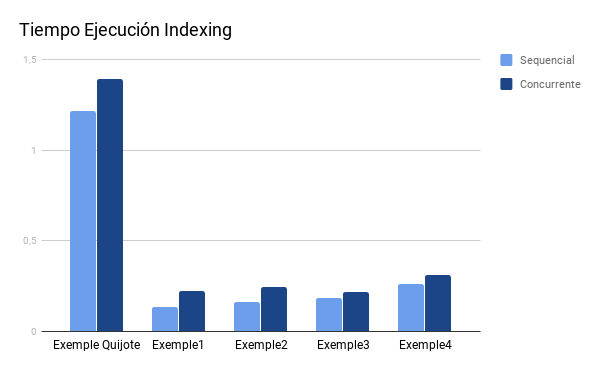
\includegraphics[width=\linewidth]{Indexing.png}
  \caption{Indexing}
  \label{fig:indexing}
\end{figure}
\begin{figure}[hbt!]
  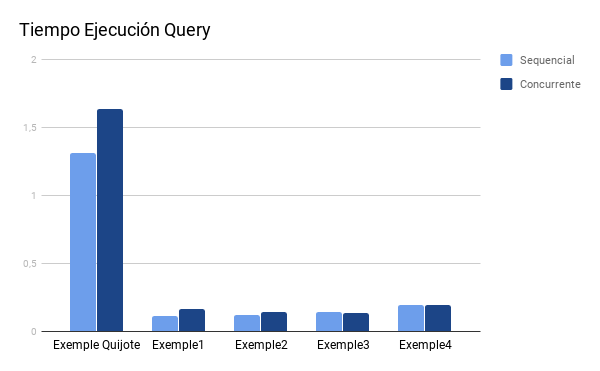
\includegraphics[width=\linewidth]{Query.png}
  \caption{Query}
  \label{fig:query}
\end{figure}
\newpage
%escriure a partir d'aquí
El objetivo de la práctica ha sido implementar la versión concurrente de 
Query y Indexing, así como estudiar su comportamiento y tiempos de ejecución.
\\\\ 
En las gráficas se pueden discernir los tiempos de ejecución
de cada uno de los ejemplos en su versión secuencial y concurrente, sin embargo, cabe destacar algunas peculiaridades sobre los resultados obtenidos.\\
\\
El resultado más destacable es que en algunos casos la aplicación concurrente nos da un tiempo superior a la implementación secuencial, y esto se debe por lo siguiente:
Nuestra implementación tanto en Query como en Indexing se basa en una estrategia Master/Worker que consiste en dividir la construcción del HashMap de Inverted Index en diferentes hilos, haciendo que cada hilo construya su propio HashMap. Posteriormente unimos los HashMaps de cada uno de los hilos para generar el definitivo. Esta última operación genera un cuello de botella haciéndola bastante costosa en tiempo, cosa que explica porque a veces la aplicación concurrente es menos eficiente que la secuencial.

\section{Diferencias entre multiples hilos}
\begin{figure}[hbt!]
  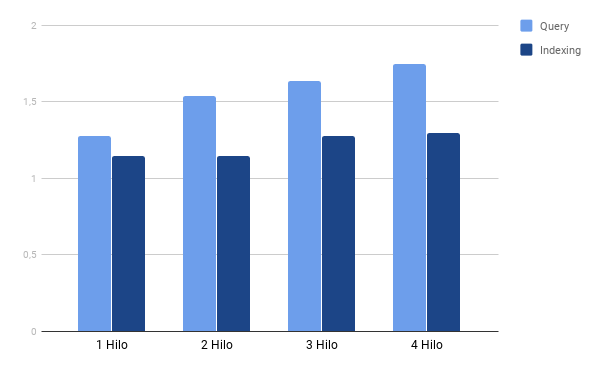
\includegraphics[width=\linewidth]{multithreading.png}
  \caption{Ejecucion con múltiples hilos}
  \label{fig:multhilos}
\end{figure}

Como se puede ver en la Figura \ref{fig:multhilos}, en el caso tanto de Query como de Indexing conforme mas hilos ejecutándose de forma paralela, más coste en el tiempo.\\
Esto es debido a lo ya mencionado en el apartado anterior, a más hilos más veces se tiene que realizar la operación putAll alargando más el cuello de botella.\\

\section{Diseño de la Solución}
La solución presentada en esta práctica consiste en lo siguiente.
\subsection{Indexing}
Se reciben por parámetro el número de hilos con los que se desea ejecutar la aplicación. Con este se realiza un balanceo de carga asignando a cada hilo un número determinado de caracteres a procesar del fichero. Una vez asignado a cada hilo la carga de trabajo a realizar, estos empiezan a procesar carácter a carácter las claves i a construir su propio HashMap. Una vez realizado el join de todos los hilos, se juntan los HashMaps parciales en uno global i se continua con la ejecución del programa.
%TODO: Si vols, explicar lo de la mierda de Save Index així una mica per demunt i lo del cuello de botella de remove
\subsection{Query}
Utiliza la misma estructura que Indexing, pero esta vez el balanceo de carga se realiza respecto a los ficheros que deben leer cada uno de los hilos. Entonces cada thread leerà un número de fitxeros y creará su propio hashmap así continuando con el mismo proceso que Indexing.

\end{document}

